% answers.tex —— 2003 年·北京卷·理科 · 参考答案与详细解析片段
% 由 tools/generate_projects.py 依来源总账自 2003/2003_数学真题_北京理_试题.md + 2003/2003_数学真题_北京理_解析正文.md + 2003/2003_数学真题_北京理_答案要点.md 生成，勿手改（改源 MD 后重跑）


\begin{gktip}
固定候选 PDF 仅含题面；以下解析依据已复核题面独立推导，属于本库非官方内容。来源身份与官方答案未核，\texttt{official_answer=null}。Q17 照录“底面边长的 3”，不补“为”；题设不足时不把条件性推导写成确定答案。
\end{gktip}

\gkpart{一、选择题}

\begin{answer}
\gksolhead{1}{}

\textbf{题目}：

\Needspace{5\baselineskip}
设集合
\nopagebreak[4]
\[
   A=\{x\mid x^2-1>0\},\qquad B=\{x\mid \log_2x>0\},
\]
   (A\cap B) 等于\mbox{（　　）}

   (A) \(\{x\mid x>1\}\)　　(B) \(\{x\mid x>0\}\)

   (C) \(\{x\mid x<-1\}\)　　(D) \(\{x\mid x<-1\text{ 或 }x>1\}\)

\Needspace{4\baselineskip}
\textbf{解析}

由 \(x^2-1>0\) 得 \(x<-1\) 或 \(x>1\)，而 \(\log_2x>0\) 要求 \(x>1\)，交集为 \(x>1\)，选 A。

\gkanswer{答案：A}

\end{answer}
\begin{answer}
\gksolhead{2}{}

\textbf{题目}：

\Needspace{5\baselineskip}
设
\nopagebreak[4]
\[
   y_1=4^{0.9},\qquad y_2=8^{0.44},\qquad y_3=\left(\frac12\right)^{-1.5},
\]
   则\mbox{（　　）}

   (A) \(y_3>y_1>y_2\)　　(B) \(y_2>y_1>y_3\)

   (C) \(y_1>y_2>y_3\)　　(D) \(y_1>y_3>y_2\)

\Needspace{4\baselineskip}
\textbf{解析}

\nopagebreak[4]
\[
y_1=2^{1.8},\quad y_2=2^{1.32},\quad y_3=2^{1.5}
\]
。
故 \(y_1>y_3>y_2\)，选 D。

\gkanswer{答案：D}

\end{answer}
\begin{answer}
\gksolhead{3}{}

\textbf{题目}：

“\(\cos 2\alpha=-\dfrac{\sqrt3}{2}\)”是“\(\alpha=k\pi+\dfrac{5\pi}{12},\ k\in\mathbb Z\)”的\mbox{（　　）}

   (A) 必要非充分条件　　(B) 充分非必要条件

   (C) 充分必要条件　　(D) 既非充分又非必要条件

\Needspace{4\baselineskip}
\textbf{解析}

若 \(\alpha=k\pi+5\pi/12\)，则 \(\cos2\alpha=-\sqrt3/2\)，故给定角度形式是该余弦等式的充分条件。反过来，余弦等式还允许 \(\alpha=k\pi+7\pi/12\)，所以它不是给定角度形式的充分条件；按题目“前者是后者的条件”判断，选 A（必要非充分）。

\gkanswer{答案：A（必要非充分条件）}

\end{answer}
\begin{answer}
\gksolhead{4}{}

\textbf{题目}：

已知 \(\alpha,\beta\) 是平面，\(m,n\) 是直线。下列命题中不正确的是\mbox{（　　）}

   (A) 若 \(m\parallel n,\ m\perp\alpha\)，则 \(n\perp\alpha\)

   (B) 若 \(m\parallel\alpha,\ \alpha\cap\beta=n\)，则 \(m\parallel n\)

   (C) 若 \(m\perp\alpha,\ m\perp\beta\)，则 \(\alpha\parallel\beta\)

   (D) 若 \(m\perp\alpha,\ m\subset\beta\)，则 \(\alpha\perp\beta\)

\Needspace{4\baselineskip}
\textbf{解析}

选项 B 不成立：直线平行于平面 \(\alpha\) 并不要求其方向与交线 \(n=\alpha\cap\beta\) 平行。其余三项为线面垂直、同垂线的两平面关系及线面垂直判定的直接性质。

\gkanswer{答案：B}

\end{answer}
\begin{answer}
\gksolhead{5}{}

\textbf{题目}：

\Needspace{5\baselineskip}
极坐标方程
\nopagebreak[4]
\[
   \rho^2\cos 2\theta-2\rho\cos\theta=1
\]
   表示的曲线是\mbox{（　　）}

   (A) 圆　　(B) 椭圆　　(C) 抛物线　　(D) 双曲线

\Needspace{4\baselineskip}
\textbf{解析}

\Needspace{5\baselineskip}
代入 \(x=\rho\cos\theta\)、\(y=\rho\sin\theta\)，原式化为
\nopagebreak[4]
\[
x^2-y^2-2x=1\quad\Longleftrightarrow\quad (x-1)^2-y^2=2,
\]
为双曲线，选 D。

\gkanswer{答案：D，双曲线}

\end{answer}
\begin{answer}
\gksolhead{6}{}

\textbf{题目}：

若 \(z\in\mathbb C\) 且 \(|z+2-2i|=1\)，则 \(|z-2-2i|\) 的最小值是\mbox{（　　）}

   (A) 2　　(B) 3　　(C) 4　　(D) 5

\Needspace{4\baselineskip}
\textbf{解析}

点 \(z\) 在以 \((-2,2)\) 为圆心、半径 1 的圆上；目标是到 \((2,2)\) 的距离。两中心相距 4，最小距离为 \(4-1=3\)，选 B。

\gkanswer{答案：B，最小值为 3}

\end{answer}
\begin{answer}
\gksolhead{7}{}

\textbf{题目}：

如果圆台的母线与底面成 \(60^\circ\) 角，那么这个圆台的侧面积与轴截面面积的比为\mbox{（　　）}

   (A) \(2\pi\)　　(B) \(\dfrac{3}{2}\pi\)　　(C) \(\dfrac{2\sqrt3}{3}\pi\)　　(D) \(\dfrac12\pi\)

\Needspace{4\baselineskip}
\textbf{解析}

设圆台两底半径为 \(R,r\)，母线长为 \(l\)，高为 \(h\)。由母线与底面成 \(60^\circ\)，\(h=l\sin60^\circ=\sqrt3l/2\)。侧面积为 \(\pi(R+r)l\)，轴截面为面积 \((R+r)h\) 的梯形，故比值 \(2\pi/\sqrt3\)，选 C。

\gkanswer{答案：C，\(\dfrac{2\sqrt3}{3}\pi\)}

\end{answer}
\begin{answer}
\gksolhead{8}{}

\textbf{题目}：

从黄瓜、白菜、油菜、扁豆 4 种蔬菜品种中选出 3 种，分别种在不同土质的三块土地上，其中黄瓜必须种植，不同的种植方法共有\mbox{（　　）}

   (A) 24 种　　(B) 18 种　　(C) 12 种　　(D) 6 种

\Needspace{4\baselineskip}
\textbf{解析}

黄瓜必须选，再从其他三种选两种，有 \(\binom32\) 种；三种蔬菜分配到三块不同土地有 \(3!\) 种，合计 18 种，选 B。

\gkanswer{答案：B，18 种}

\end{answer}
\begin{answer}
\gksolhead{9}{}

\textbf{题目}：

\Needspace{5\baselineskip}
若数列 \(\{a_n\}\) 的通项公式是
\nopagebreak[4]
\[
   a_n=\frac{3^{-n}+2^{-n}+(-1)^n(3^{-n}-2^{-n})}{2},\qquad n=1,2,\ldots,
\]
   则 \(\displaystyle\lim_{n\to\infty}(a_1+a_2+\cdots+a_n)\) 等于\mbox{（　　）}

   (A) \(\dfrac{11}{24}\)　　(B) \(\dfrac{17}{24}\)　　(C) \(\dfrac{19}{24}\)　　(D) \(\dfrac{25}{24}\)

\Needspace{4\baselineskip}
\textbf{解析}

\Needspace{5\baselineskip}
当 \(n\) 为奇数，\(a_n=2^{-n}\)；当 \(n\) 为偶数，\(a_n=3^{-n}\)。因此
\nopagebreak[4]
\[
\sum_{n=1}^{\infty}a_n=\frac{1/2}{1-1/4}+\frac{1/9}{1-1/9}=\frac23+\frac18=\frac{19}{24},
\]
选 C。

\gkanswer{答案：C，\(\dfrac{19}{24}\)}

\end{answer}
\begin{answer}
\gksolhead{10}{}

\textbf{题目}：

\Needspace{5\baselineskip}
某班试用电子投票系统选举班干部候选人。全班 \(k\) 名同学都有选举权和被选举权，他们的编号分别为 \(1,2,\ldots,k\)。规定：同意按“1”，不同意（含弃权）按“0”，令
\nopagebreak[4]
\[
    a_{ij}=\begin{cases}
    1,&\text{第 }i\text{ 号同学同意第 }j\text{ 号同学当选},\\
    0,&\text{第 }i\text{ 号同学不同意第 }j\text{ 号同学当选},
    \end{cases}
\]
    其中 \(i=1,2,\ldots,k\)，且 \(j=1,2,\ldots,k\)，则同时同意第 1、2 号同学当选的人数为\mbox{（　　）}

    (A) \(a_{11}+a_{12}+\cdots+a_{1k}+a_{21}+a_{22}+\cdots+a_{2k}\)

    (B) \(a_{11}+a_{21}+\cdots+a_{k1}+a_{12}+a_{22}+\cdots+a_{k2}\)

    (C) \(a_{11}a_{12}+a_{21}a_{22}+\cdots+a_{k1}a_{k2}\)

    (D) \(a_{11}a_{21}+a_{12}a_{22}+\cdots+a_{1k}a_{2k}\)

\Needspace{4\baselineskip}
\textbf{解析}

第 \(i\) 位同学同时同意 1、2 号当选的指示量为 \(a_{i1}a_{i2}\)，所以人数为 \(\sum_{i=1}^k a_{i1}a_{i2}\)，选 C。

\gkanswer{答案：C}

\end{answer}
\gkpart{二、填空题}

\begin{answer}
\gksolhead{11}{}

\textbf{题目}：

\Needspace{5\baselineskip}
函数
\nopagebreak[4]
\[
    f(x)=\lg(1+x^2),\qquad
    g(x)=\begin{cases}
    x+2,&x<-1,\\
    0,&|x|\le 1,\\
    -x+2,&x>1,
    \end{cases}
    \qquad h(x)=\tan 2x
\]
    中，\gkblank{} 是偶函数。

\Needspace{4\baselineskip}
\textbf{解析}

\(f(-x)=f(x)\)，且分段函数 \(g\) 在 \(|x|\le1\) 时为 0、在区间外只依赖 \(|x|\)，故 \(g(-x)=g(x)\)。而 \(h(x)=\tan2x\) 是奇函数。因此 \(f\) 与 \(g\) 都是偶函数。

\gkanswer{答案：\(f(x)\) 与 \(g(x)\)}

\end{answer}
\begin{answer}
\gksolhead{12}{}

\textbf{题目}：

\Needspace{5\baselineskip}
以双曲线
\nopagebreak[4]
\[
    \frac{x^2}{16}-\frac{y^2}{9}=1
\]
    右顶点为顶点、左焦点为焦点的抛物线的方程是\gkblank{}。

\Needspace{4\baselineskip}
\textbf{解析}

\Needspace{5\baselineskip}
双曲线焦点为 \((\pm5,0)\)，左焦点为 \((-5,0)\)；右顶点为 \((4,0)\)。抛物线顶点至焦点的有向距离参数为 \(p=-9\)，故
\nopagebreak[4]
\[
y^2=4p(x-4)=-36(x-4)
\]
。

\gkanswer{答案：\(y^2=-36(x-4)\)}

\end{answer}
\begin{answer}
\gksolhead{13}{}

\textbf{题目}：

如图，已知底面半径为 \(r\) 的圆柱被一个平面所截，剩下部分母线长的最大值为 \(a\)，最小值为 \(b\)，那么圆柱被截后剩下部分的体积是\gkblank{}。
\nopagebreak[4]
\begin{center}% Generator: hand-authored TikZ schematic traced from the fixed source; cylinder proportions are illustrative.
% Source ID: src-120ea104f8cb373f5731039fa9d36469df457869849f27420831962ef1ad2306
% PDF SHA-256: d0081500bd56d03199ddcf232fe8e870f2ecd7e9c41ba849417af9af79fbb702
% PDF page 1; printed page 124; question 13.
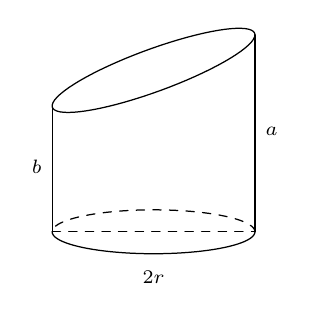
\begin{tikzpicture}[
  x=0.92cm,y=0.82cm,line width=0.45pt,line cap=round,
  every node/.style={font=\scriptsize,inner sep=1.5pt}
]
  % Lower base: dashed rear arc and diameter, solid front arc.
  \draw[dashed,domain=0:180,samples=48,variable=\t]
    plot ({1.4*cos(\t)},{0.34*sin(\t)});
  \draw[domain=180:360,samples=48,variable=\t]
    plot ({1.4*cos(\t)},{0.34*sin(\t)});
  \draw[dashed] (-1.4,0)--(1.4,0);

  % Oblique cut ellipse: the right generator is longer than the left one.
  \draw[domain=0:360,samples=72,variable=\t]
    plot ({1.4*cos(\t)},{2.5+0.55*cos(\t)+0.35*sin(\t)});
  \draw (-1.4,0)--(-1.4,1.95) (1.4,0)--(1.4,3.05);

  \node[left] at (-1.48,1.0) {$b$};
  \node[right] at (1.48,1.55) {$a$};
  \node[below] at (0,-0.54) {$2r$};
\end{tikzpicture}
\end{center}
\nopagebreak[4]
\Needspace{4\baselineskip}
\textbf{解析}

\Needspace{5\baselineskip}
将底面圆盘上的坐标记为 \((x,y)\)。截平面与圆盘平面的高度差是 \((x,y)\) 的仿射函数。圆盘关于圆心中心对称，仿射函数在圆盘上的平均值等于其中心值；由直径两端最大、最小母线长为 \(a,b\)，中心高度为 \((a+b)/2\)。故剩余体积为
\nopagebreak[4]
\[
V=\pi r^2\frac{a+b}{2}
\]
。

\gkanswer{答案：\(V=\dfrac{\pi r^2(a+b)}2\)}

\end{answer}
\begin{answer}
\gksolhead{14}{}

\textbf{题目}：

将长度为 1 的铁丝分成两段，分别围成一个正方形和一个圆形，要使正方形与圆的面积之和最小，正方形的周长应为\gkblank{}。

\Needspace{4\baselineskip}
\textbf{解析}

\Needspace{5\baselineskip}
设正方形周长为 \(s\in[0,1]\)，面积和为
\nopagebreak[4]
\[
S(s)=\frac{s^2}{16}+\frac{(1-s)^2}{4\pi}
\]
。
由 \(S'(s)=s/8-(1-s)/(2\pi)=0\) 得 \(s=4/(4+\pi)\)。二阶导数为正，故为最小值点。

\gkanswer{答案：\(\dfrac4{4+\pi}\)}

\end{answer}
\gkpart{三、解答题}

\begin{answer}
\gksolhead{15}{}

\textbf{题目}：

\Needspace{5\baselineskip}
已知函数
\nopagebreak[4]
\[
    f(x)=\cos^4x-2\sin x\cos x-\sin^4x.
\]

    (1) 求 \(f(x)\) 的最小正周期；

    (2) 若 \(x\in\left[0,\dfrac{\pi}{2}\right]\)，求 \(f(x)\) 的最大值、最小值。

\Needspace{4\baselineskip}
\textbf{解析}

\gksubpart{(1) 最小正周期}

\Needspace{5\baselineskip}
化简得
\nopagebreak[4]
\[
f(x)=\cos2x-\sin2x=\sqrt2\cos(2x+\pi/4),
\]
故最小正周期为 \(\pi\)。

\gksubpart{(2) 最大值与最小值}

令 \(t=2x\in[0,\pi]\)，则 \(f=\cos t-\sin t\)。端点值为 1、$-$1；唯一内部驻点为 \(t=3\pi/4\)，函数值为 \(-\sqrt2\)。因此最大值 1，最小值 \(-\sqrt2\)。

\gkanswer{答案（1）：最小正周期为 \(\pi\)}

\gkanswer{答案（2）：最大值为 1，最小值为 \(-\sqrt2\)}

\end{answer}
\begin{answer}
\gksolhead{16}{}

\textbf{题目}：

已知数列 \(\{a_n\}\) 是等差数列，且 \(a_1=2,\ a_1+a_2+a_3=12\)。

    (1) 求数列 \(\{a_n\}\) 的通项公式；

    (2) 令 \(b_n=a_nx^n\ (x\in\mathbb R)\)。求数列 \(\{b_n\}\) 前 \(n\) 项和的公式。

\Needspace{4\baselineskip}
\textbf{解析}

\gksubpart{(1) 求通项}

等差数列前三项和为 \(3a_1+3d=12\)，由 \(a_1=2\) 得 \(d=2\)，故 \(a_n=2n\)。

\gksubpart{(2) 求前 n 项和}

\Needspace{5\baselineskip}
\(b_k=2kx^k\)。当 \(x=1\)，\(S_n=2\sum_{k=1}^n k=n(n+1)\)。当 \(x\ne1\)，由有限几何级数求导，
\nopagebreak[4]
\[
S_n=2\sum_{k=1}^n kx^k=\frac{2x\bigl(1-(n+1)x^n+nx^{n+1}\bigr)}{(1-x)^2}
\]
。

\gkanswer{答案（1）：\(a_n=2n\)}

\gkanswer{答案（2）：\(x=1\) 时 \(S_n=n(n+1)\)；\(x\ne1\) 时 \(S_n=\dfrac{2x(1-(n+1)x^n+nx^{n+1})}{(1-x)^2}\)}

\end{answer}
\begin{answer}
\gksolhead{17}{}

\textbf{题目}：

如图，正三棱柱 \(ABC-A_1B_1C_1\) 的底面边长的 3，侧棱 \(AA_1=\dfrac{3\sqrt3}{2}\)，\(D\) 是 \(CB\) 延长线上一点，且 \(BD=BC\)。

\begin{gktip}
原页疑点（待核）：原页可见字面为“底面边长的 3”，语句不完整，未见“为”；本稿照录，不按语义补字。
\end{gktip}

    (1) 求证：直线 \(BC_1\parallel\) 平面 \(AB_1D\)；

    (2) 求二面角 \(B_1-AD-B\) 的大小；

    (3) 求三棱锥 \(C_1-ABB_1\) 的体积。
\nopagebreak[4]
\begin{center}% Generator: hand-authored TikZ schematic traced from source-visible edges and labels; projection is illustrative.
% Source ID: src-120ea104f8cb373f5731039fa9d36469df457869849f27420831962ef1ad2306
% PDF SHA-256: d0081500bd56d03199ddcf232fe8e870f2ecd7e9c41ba849417af9af79fbb702
% PDF page 1; printed page 124; question 17.
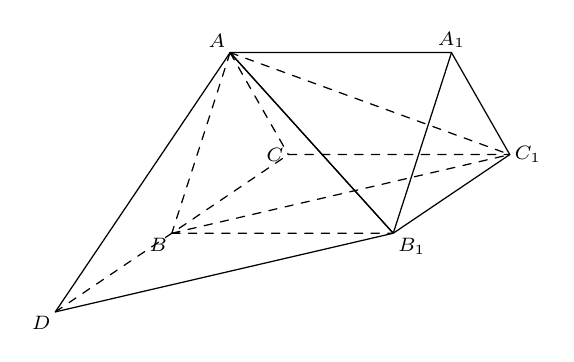
\begin{tikzpicture}[
  x=0.74cm,y=0.74cm,line width=0.45pt,line cap=round,line join=round,
  every node/.style={font=\scriptsize,inner sep=1.5pt}
]
  \coordinate (A)  at (0.7,4.2);
  \coordinate (A1) at (4.5,4.2);
  \coordinate (B)  at (-0.3,1.1);
  \coordinate (B1) at (3.5,1.1);
  \coordinate (C)  at (1.7,2.45);
  \coordinate (C1) at (5.5,2.45);
  \coordinate (D)  at (-2.3,-0.25);

  % Source-visible prism and auxiliary edges.
  \draw (D)--(A) (D)--(B1) (A)--(B1);
  \draw (A)--(A1)--(C1)--(B1)--cycle;
  \draw (A1)--(B1);
  \draw[dashed] (D)--(B)--(C) (A)--(B) (A)--(C);
  \draw[dashed] (A)--(C1) (B)--(B1) (B)--(C1) (C)--(C1);

  \node[above left] at (A) {$A$};
  \node[above] at (A1) {$A_1$};
  \node[below left] at (B) {$B$};
  \node[below right] at (B1) {$B_1$};
  \node[left] at (C) {$C$};
  \node[right] at (C1) {$C_1$};
  \node[below left] at (D) {$D$};
\end{tikzpicture}
\end{center}
\nopagebreak[4]
\Needspace{4\baselineskip}
\textbf{解析}

\Needspace{5\baselineskip}
原页字面为“底面边长的 3”，未见关系词“为”。令实际底面边长为未知 \(s>0\)，侧棱长 \(h=3\sqrt3/2\)，取
\nopagebreak[4]
\[
B=(0,0,0),\ C=(s,0,0),\ A=(s/2,\sqrt3s/2,0),\ D=(-s,0,0),\ B_1=(0,0,h),\ C_1=(s,0,h)
\]
。

\gksubpart{(1) 证明线面平行}

\Needspace{5\baselineskip}
令 \(u=\overrightarrow{AB_1}=(-s/2,-\sqrt3s/2,h)\)、\(v=\overrightarrow{AD}=(-3s/2,-\sqrt3s/2,0)\)。平面 \(AB_1D\) 的法向量可取
\nopagebreak[4]
\[
u\times v=(\sqrt3hs/2,-3hs/2,-\sqrt3s^2/2)
\]
。
\(\overrightarrow{BC_1}=(s,0,h)\) 与该法向量点积为 0；且 B 不在平面 \(AB_1D\) 上。因此 \(BC_1\parallel\) 平面 \(AB_1D\)。此结论不依赖 s。

\gksubpart{(2) 求二面角}

\Needspace{5\baselineskip}
将从棱 \(AD\) 指向 B、\(B_1\) 的向量投影到垂直于 \(AD\) 的平面，所得二面角 \(\theta\) 满足
\nopagebreak[4]
\[
\cos\theta=\frac{s}{\sqrt{s^2+4h^2}}
\]
。
故未知底面边长会改变角度。若条件性假设 \(s=3\)，则 \(\theta=60^\circ\)；此值不是当前题面确定给出的答案。

\gksubpart{(3) 求三棱锥体积}

\Needspace{5\baselineskip}
以三角形 \(ABB_1\) 为底，面积为 \(sh/2\)。点 \(C_1\) 到平面 \(ABB_1\) 的距离为等边三角形中 C 到 AB 的距离 \(\sqrt3s/2\)，所以
\nopagebreak[4]
\[
V=\frac13\cdot\frac{sh}{2}\cdot\frac{\sqrt3s}{2}=\frac{3s^2}{8}
\]
。
仅在条件性假设 \(s=3\) 时，\(V=27/8\)。

\gkanswer{答案（1）：\(BC_1\parallel\) 平面 \(AB_1D\)}

\gkanswer{答案（2）：U/PENDING；若另有证据确认底面边长 \(s=3\)，条件性结果为 \(60^\circ\)}

\gkanswer{答案（3）：U/PENDING；若另有证据确认底面边长 \(s=3\)，条件性结果为 \(V=27/8\)}

\end{answer}
\begin{answer}
\gksolhead{18}{}

\textbf{题目}：

如图，椭圆的长轴 \(A_1A_2\) 与 \(x\) 轴平行，短轴 \(B_1B_2\) 在 \(y\) 轴上，中心为 \(M(0,r)\)（\(b>r>0\)）。

    (1) 写出椭圆的方程，求椭圆的焦点坐标及离心率；

\Needspace{5\baselineskip}
    (2) 直线 \(y=k_1x\) 交椭圆于两点 \(C(x_1,y_1),D(x_2,y_2)\)（\(y_2>0\)）；直线 \(y=k_2x\) 交椭圆于两点 \(G(x_3,y_3),H(x_4,y_4)\)（\(y_4>0\)）。求证：
\nopagebreak[4]
\[
    \frac{k_1x_1x_2}{x_1+x_2}=\frac{k_2x_3x_4}{x_3+x_4};
\]

    (3) 对于 (2) 中的 \(C,D,G,H\)，设 \(CH\) 交 \(x\) 轴于点 \(P\)，\(GD\) 交 \(x\) 轴于点 \(Q\)。求证：\(|OP|=|OQ|\)。（证明过程不考虑 \(CH\) 或 \(GD\) 垂直于 \(x\) 轴的情形。）
\nopagebreak[4]
\begin{center}% Generator: hand-authored TikZ schematic traced from the fixed source; ellipse and chord coordinates are illustrative.
% Source ID: src-120ea104f8cb373f5731039fa9d36469df457869849f27420831962ef1ad2306
% PDF SHA-256: d0081500bd56d03199ddcf232fe8e870f2ecd7e9c41ba849417af9af79fbb702
% PDF page 2; printed page 125; question 18.
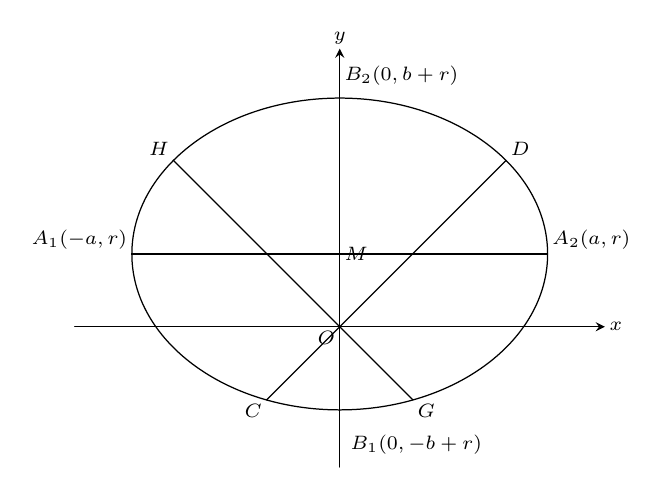
\begin{tikzpicture}[
  x=0.66cm,y=0.66cm,line width=0.45pt,line cap=round,>=stealth,
  every node/.style={font=\scriptsize,inner sep=1.5pt}
]
  \coordinate (O)  at (0,0);
  \coordinate (M)  at (0,1.4);
  \coordinate (A1) at (-4,1.4);
  \coordinate (A2) at (4,1.4);
  \coordinate (B1) at (0,-1.6);
  \coordinate (B2) at (0,4.4);
  \coordinate (H)  at (-3.2,3.2);
  \coordinate (G)  at (1.408,-1.408);
  \coordinate (C)  at (-1.408,-1.408);
  \coordinate (D)  at (3.2,3.2);

  \draw[->] (-5.1,0)--(5.1,0) node[right] {$x$};
  \draw[->] (0,-2.7)--(0,5.35) node[above] {$y$};
  \draw (M) ellipse [x radius=4,y radius=3];
  \draw (A1)--(A2);
  \draw (H)--(G) (C)--(D);

  \node[above left] at (A1) {$A_1(-a,r)$};
  \node[above right] at (A2) {$A_2(a,r)$};
  \node[above right] at (0,4.55) {$B_2(0,b+r)$};
  \node[below right] at (0.12,-2.0) {$B_1(0,-b+r)$};
  \node[right] at (M) {$M$};
  \node[below left] at (O) {$O$};
  \node[above left] at (H) {$H$};
  \node[below right] at (G) {$G$};
  \node[below left] at (C) {$C$};
  \node[above right] at (D) {$D$};
\end{tikzpicture}
\end{center}
\nopagebreak[4]
\Needspace{4\baselineskip}
\textbf{解析}

\gksubpart{(1) 椭圆方程、焦点与离心率}

\Needspace{5\baselineskip}
椭圆中心为 \(M(0,r)\)，长轴水平、短轴竖直，故
\nopagebreak[4]
\[
\frac{x^2}{a^2}+\frac{(y-r)^2}{b^2}=1,\quad c=\sqrt{a^2-b^2}
\]
。
焦点为 \((\pm c,r)\)，离心率 \(e=c/a\)。

\gksubpart{(2) 证明比值相等}

\Needspace{5\baselineskip}
将 \(y=kx\) 代入椭圆，交点横坐标是二次方程
\nopagebreak[4]
\[
\left(\frac1{a^2}+\frac{k^2}{b^2}\right)x^2-\frac{2rk}{b^2}x+\left(\frac{r^2}{b^2}-1\right)=0
\]
\Needspace{5\baselineskip}
的两根 \(x_1,x_2\)。由韦达定理，
\nopagebreak[4]
\[
x_1+x_2=\frac{2rk/b^2}{1/a^2+k^2/b^2},\qquad x_1x_2=\frac{r^2/b^2-1}{1/a^2+k^2/b^2}
\]
。
\Needspace{5\baselineskip}
因此
\nopagebreak[4]
\[
\frac{kx_1x_2}{x_1+x_2}=\frac{r^2-b^2}{2r},
\]
与 k 无关。

\gksubpart{(3) 证明两段长度相等}

\Needspace{5\baselineskip}
记 \(P=(p,0),Q=(q,0)\)。直线截距公式给出
\nopagebreak[4]
\[
p=\frac{x_1x_4(k_2-k_1)}{k_2x_4-k_1x_1},\qquad q=\frac{x_2x_3(k_2-k_1)}{k_2x_3-k_1x_2}
\]
。
\Needspace{5\baselineskip}
由（2）两直线共有常数 \(K\)，即 \(k_1x_1x_2=K(x_1+x_2)\)、\(k_2x_3x_4=K(x_3+x_4)\)。通分后有
\nopagebreak[4]
\[
p+q=\frac{(k_2-k_1)\left[x_1x_4(k_2x_3-k_1x_2)+x_2x_3(k_2x_4-k_1x_1)\right]}{(k_2x_4-k_1x_1)(k_2x_3-k_1x_2)}
\]
。
\Needspace{5\baselineskip}
方括号中的项等于
\nopagebreak[4]
\[
k_2x_3x_4(x_1+x_2)-k_1x_1x_2(x_3+x_4)=0,
\]
由共有常数 \(K\) 可知该等式成立。因此 \(p+q=0\)，从而 \(|OP|=|p|=|q|=|OQ|\)。

\gkanswer{答案（1）：\(\dfrac{x^2}{a^2}+\dfrac{(y-r)^2}{b^2}=1\)，焦点为 \((\pm\sqrt{a^2-b^2},r)\)，离心率为 \(\dfrac{\sqrt{a^2-b^2}}a\)}

\gkanswer{答案（2）：\(\dfrac{kx_1x_2}{x_1+x_2}=\dfrac{r^2-b^2}{2r}\)}

\gkanswer{答案（3）：\(|OP|=|OQ|\)}

\end{answer}
\begin{answer}
\gksolhead{19}{}

\textbf{题目}：

有三个新兴城镇，分别位于 \(A,B,C\) 三点处，且 \(AB=AC=a,\ BC=2b\)。今计划合建一个中心医院，为同时方便三镇，准备建在 \(BC\) 的垂直平分线上的 \(P\) 点处。（建立坐标系如图）

    (1) 若希望点 \(P\) 到三镇距离的平方和为最小，点 \(P\) 应位于何处？

    (2) 若希望点 \(P\) 到三镇的最远距离为最小，点 \(P\) 应位于何处？
\nopagebreak[4]
\begin{center}% Generator: hand-authored TikZ schematic traced from the fixed source; triangle proportions are illustrative.
% Source ID: src-120ea104f8cb373f5731039fa9d36469df457869849f27420831962ef1ad2306
% PDF SHA-256: d0081500bd56d03199ddcf232fe8e870f2ecd7e9c41ba849417af9af79fbb702
% PDF page 2; printed page 125; question 19.
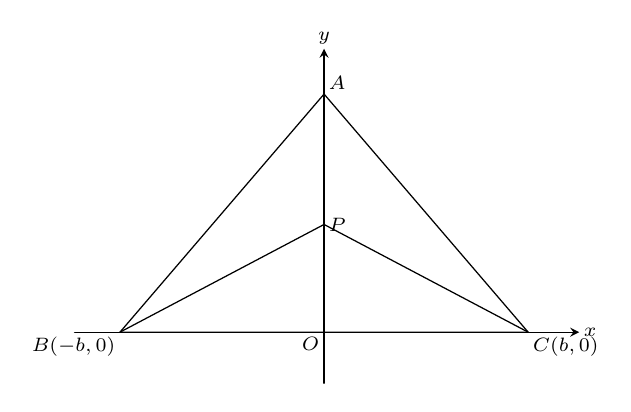
\begin{tikzpicture}[
  x=0.72cm,y=0.72cm,line width=0.45pt,line cap=round,>=stealth,
  every node/.style={font=\scriptsize,inner sep=1.5pt}
]
  \coordinate (O) at (0,0);
  \coordinate (A) at (0,4.2);
  \coordinate (P) at (0,1.9);
  \coordinate (B) at (-3.6,0);
  \coordinate (C) at (3.6,0);

  \draw[->] (-4.4,0)--(4.5,0) node[right] {$x$};
  \draw[->] (0,-0.9)--(0,5.0) node[above] {$y$};
  \draw (A)--(B)--(C)--cycle;
  \draw (P)--(B) (P)--(C);

  \node[above right] at (A) {$A$};
  \node[below left] at (B) {$B(-b,0)$};
  \node[below right] at (C) {$C(b,0)$};
  \node[below left] at (O) {$O$};
  \node[right] at (P) {$P$};
\end{tikzpicture}
\end{center}
\nopagebreak[4]
\Needspace{4\baselineskip}
\textbf{解析}

令 \(h=\sqrt{a^2-b^2}\)，取 \(B=(-b,0),C=(b,0),A=(0,h)\)，并设 \(P=(0,t)\)。

\gksubpart{(1) 最小化距离平方和}

\Needspace{5\baselineskip}
距离平方和为
\nopagebreak[4]
\[
PA^2+PB^2+PC^2=(t-h)^2+2(t^2+b^2)=3(t-h/3)^2+2b^2+2h^2/3,
\]
故在 \(t=h/3\) 取最小。

\gksubpart{(2) 最小化最远距离}

\Needspace{5\baselineskip}
三镇距离分别为 \(|h-t|\)、\(\sqrt{b^2+t^2}\)、\(\sqrt{b^2+t^2}\)。若 \(h\le b\)，在 \(t=0\) 最大距离为 b，而任何 \(t\ne0\) 到 B、C 的距离已大于 b，所以最优点为 O。若 \(h>b\)，在 \([0,h]\) 上前者递减、后者递增，令其相等得
\nopagebreak[4]
\[
h-t=\sqrt{b^2+t^2}\quad\Longrightarrow\quad t=\frac{h^2-b^2}{2h}
\]
。
两函数的最大值在该交点最小；区间外不能取得更小最大值。因此分段结果为题面速查表所列。

\gkanswer{答案（1）：\(P=(0,h/3)\)，其中 \(h=\sqrt{a^2-b^2}\)}

\gkanswer{答案（2）：\(h\le b\) 时 \(P=O\)；\(h>b\) 时 \(P=(0,\dfrac{h^2-b^2}{2h})\)}

\end{answer}
\begin{answer}
\gksolhead{20}{}

\textbf{题目}：

设 \(y=f(x)\) 是定义在区间 \([-1,1]\) 上的函数，且满足条件：

    ① \(f(-1)=f(1)=0\)；

    ② 对任意的 \(u,v\in[-1,1]\)，都有 \(|f(u)-f(v)|\le |u-v|\)。

    (1) 证明：对任意的 \(x\in[-1,1]\)，\(x-1\le f(x)\le 1-x\)；

    (2) 证明：对任意的 \(u,v\in[-1,1]\)，\(|f(u)-f(v)|\le 1\)；

\Needspace{5\baselineskip}
    (3) 在区间 \([-1,1]\) 上是否存在满足题设条件的奇函数 \(y=f(x)\)，且使得
\nopagebreak[4]
\[
    \begin{cases}
    |f(u)-f(v)|<|u-v|,&u,v\in\left[0,\dfrac12\right],\\
    |f(u)-f(v)|=|u-v|,&u,v\in\left[\dfrac12,1\right]?
    \end{cases}
\]
    若存在，请举一例；若不存在，请说明理由。

\Needspace{4\baselineskip}
\textbf{解析}

\gksubpart{(1) 证明函数值范围}

取条件②中的一端点 \(v=1\)，结合 \(f(1)=0\)，得 \(|f(x)|\le1-x\)，即 \(x-1\le f(x)\le1-x\)。

\gksubpart{(2) 证明差值上界}

\Needspace{5\baselineskip}
条件给出 \(|f(u)-f(v)|\le|u-v|\)。又端点条件推出 \(|f(x)|\le1-|x|\)。若 \(d=|u-v|\)，则
\nopagebreak[4]
\[
|f(u)-f(v)|\le\min\{d,2-|u|-|v|\}\le\min\{d,2-d\}\le1,
\]
故命题成立。

\gksubpart{(3) 判断奇函数是否存在}

奇函数满足 \(f(0)=0\)。由第二段等距条件取 \(u=1/2,v=1\)，且 \(f(1)=0\)，得 \(|f(1/2)|=1/2\)。但第一段严格不等式取 \(u=0,v=1/2\)，要求 \(|f(1/2)-f(0)|<1/2\)，矛盾，故不存在。

\gkanswer{答案（1）：\(x-1\le f(x)\le1-x\)}

\gkanswer{答案（2）：\(|f(u)-f(v)|\le1\)}

\gkanswer{答案（3）：不存在满足条件的奇函数}

\end{answer}